\section{Exercises}
\label{section:datapathControl}
\graphicspath{ {./chapter08/FigHw} }

\begin{enumerate}
\item \textbf{ (4 pts.)}
Show how to eliminate the 4-bit 2:1 mux in the bit counter by
assuming that the Y register had an asynchronous active low reset input.
Consider the fact that the external world still needs the ability to hit
a single button to reset the state of the entire circuit. 

\item  \textbf{ (6 pts.)}
A control unit has been built with the following control word:

\begin{tabular}{|c|c|c|c|c|}  \hline
Reg A       & Reg B         &  Reg P        & P mux         \\ \hline
00 hold     & 00 hold       &  1 hold       & 1 Load 0      \\ \hline
11 lsr      & 11 lsr        &               &               \\ \hline
10 lsl      & 10 lsl        &  0 load       & 0 Load Add    \\ \hline
01 load     & 01 load       &               &               \\ \hline 
\end{tabular}

Regrettably, these setting were completely wrong.  In reality here is what the control word should
have been:

\begin{tabular}{|c|c|c|c|c|}  \hline
Reg A       & Reg B         &  Reg P        & P mux         \\ \hline
00 hold     & 00 hold       &  0 hold       & 0 Load 0      \\ \hline
01 lsr      & 01 lsr        &               &               \\ \hline
10 lsl      & 10 lsl        &  1 load       & 1 Load Add    \\ \hline
11 load     & 11 load       &               &               \\ \hline 
\end{tabular}

The design team is in a total panic.
The design team thinks that it will take weeks to straighten out the error, 
they claim that the control unit needs to be redesigned.  However, there is
a cheap and easy solution.  Design some combinational 
logic to insert between the faulty control unit and the datapath in order
to straighten out the bum control signals.  There is one error can be 
fixed by changing something in the datapath, no extra hardware is 
required.  Identify this error and its solution.

\item \textbf{ (8 pts.)}
Modify the algorithm for the bit counting circuit so that it uses a 
two-line handshake to transmit the Y register.  The circuit should take
the role of an active producer in the transmission of Y.  The circuit
has four handshaking lines and two data lines.  Hint, a common
error of students is to insert a three-state buffer on the output of
the Y register to the outside world to prevent its transmission to
the outside world until the value of Y is finalized.  Don't do this!
If the outside world reads the value of Y before the circuit's signals
are valid (via the send\_REQ signal) then its their own dumb fault.
Just send the Y signal outside the datapath as is.

\item \textbf{ (16 pts.)} 
A 8kx32 RAM is full of integer data.  Design a circuit to scan
the RAM and find its smallest value.  

Turn in; an algorithm the datapath and control unit, the control word 
table, the memory input equations, and output equations.  
The control unit is to be implemented using a ones hot encoding.


\item \textbf{ (16 pts.)}
A 8kx32 RAM is full of integer data.  Design a
circuit that determines the sum of the integers {\em between} addresses
A and B.  The values of A and B are to be read in using a two-line
handshake where the circuit is to act as a passive consumer.  
The sum is to be placed in a 32-bit register S.
Turn in; an algorithm the datapath and control unit, the control word 
table, the memory input equations, and output equations.  
The control unit is to be implemented using a ones hot encoding.

\begin{onlysolution}  \textbf{Solution} \itshape{

\textbf{ Algorithm}

while(REQ==0); \\
A = datain; \\
ACK=1; \\
while(REQ==1); \\
ACK=0; \\
while(REQ==0); \\
B = datain; \\
ACK=1; \\
while(REQ==1); \\
ACK=0; \\
S=0; \\
for(i=A; i<B; i++)  { \\
 MBR=RAM[i]; \\
 S=S+MBR; \\
} // end for \\

\textbf{ DP \& CU}

\begin{figure}[ht]
\center{\scalebox{0.7}{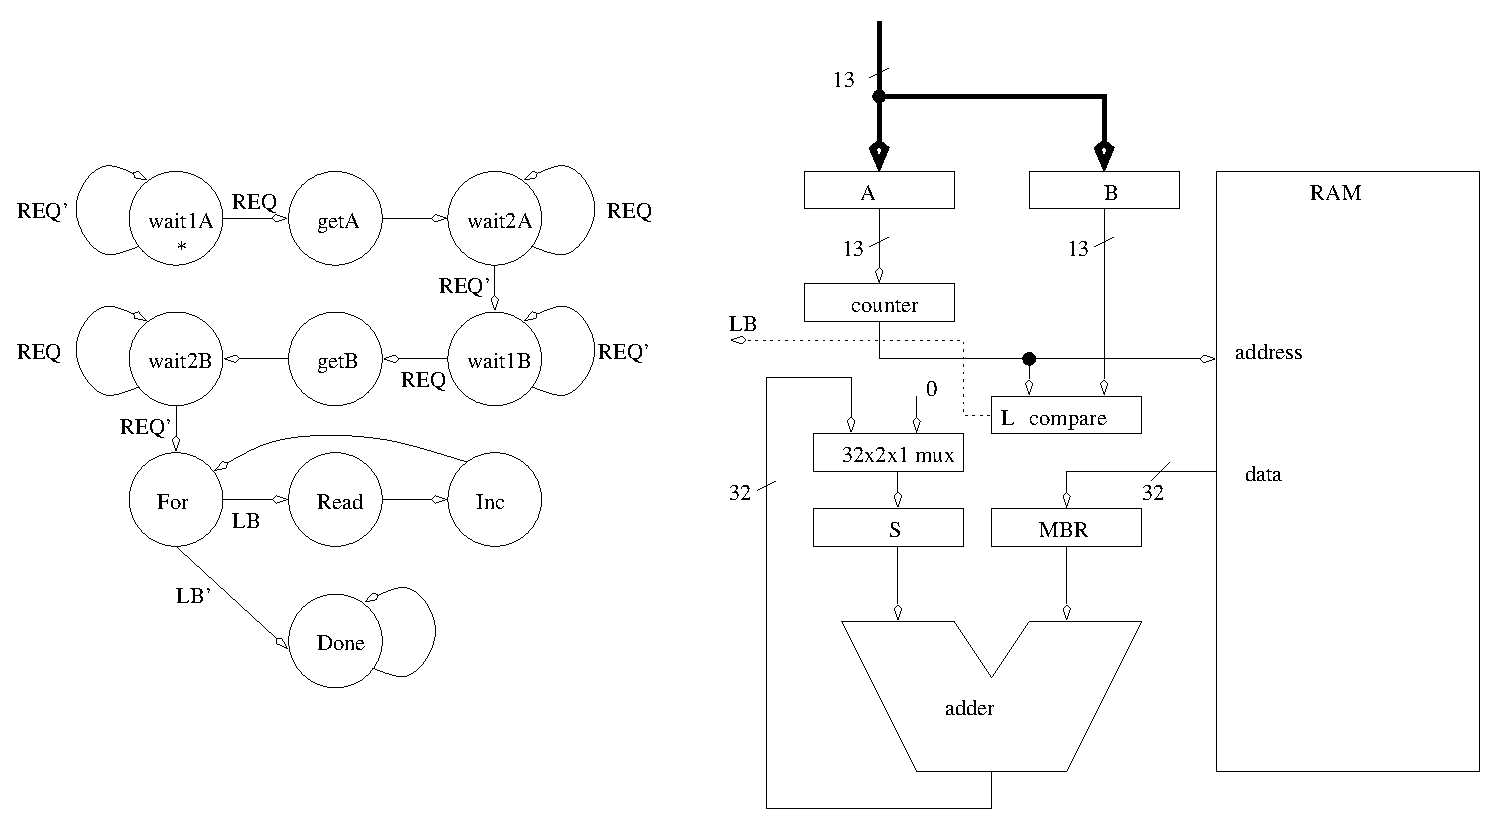
\includegraphics{Sol8-5}}}
\caption{The datapath and control to determine the sum between
addresses A and B.}
\end{figure}


\textbf{ Control Word}

\begin{tabular}{l|l|l|l|l|l|l}
STATE & A      & B      &MUX          &S      &MBR    &counter	\\ \hline
      & 0 hold & 0 hold &0 pass 0     &0 hold &0 hold &00 hold	\\ \hline
      & 1 load & 1 load &1 pass S+MBR &1 load &1 load &01 UP	\\ \hline
      &        &        &             &       &       &10 load	\\ \hline
Wait1A& 0      & 0      &0            &0      &0      &00	\\ \hline
GetA  & 1      & 0      &0            &0      &0      &00	\\ \hline
Wait2A& 0      & 0      &0            &0      &0      &00	\\ \hline
Wait1B& 0      & 0      &0            &0      &0      &00	\\ \hline
GetB  & 0      & 1      &1            &1      &0      &10	\\ \hline
Wait2B& 0      & 0      &0            &0      &0      &00	\\ \hline
For   & 0      & 0      &0            &0      &0      &00	\\ \hline
Read  & 0      & 0      &0            &0      &1      &01	\\ \hline
Inc   & 0      & 0      &1            &1      &0      &00	\\ \hline
Done  & 0      & 0      &0            &0      &0      &00	\\ 
\end{tabular}

\textbf{ MIEs and OEs}

\begin{tabular}{ll}
MIE					&	OE			\\
$D_{Wait1a}= Q_{wait1a}req'$		&  $Z_{A} = Q_{getA}$		\\
$D_{GetA } = Q_{wait1a}req$		&  $Z_{B} = Q_{getB}$		\\
$D_{wait2a}= Q_{getA} + Q_{wait2A}req$	&  $Z_{MUX} = Q_{getB} + Q_{Inc}$		\\
$D_{wait1b}= Q_{wait2a}req' + Q_{wait1B}req'$	&  $Z_{S} = Q_{getB} + Q_{Inc}$		\\
$D_{GetB } = Q_{wait1b}req$		&  $Z_{MBR} = Q_{Read}$		\\
$D_{wait2B}= Q_{GetB} + Q_{wait2b}req$	&  $Z_{c1} = Q_{GetB}$		\\
$D_{For  } = Q_{wait2B}req'$		&  $Z_{c0} = Q_{Read}$		\\
$D_{Read } = Q_{For}LB$			&  		\\
$D_{Inc  } = Q_{Read}$			& 		\\
$D_{Done } = Q_{For}LB'$		&  		\\
\end{tabular}

} \end{onlysolution} 

\item  \textbf{ (16 pts.)}
Design a circuit that repetitively looks at a 1-bit input X.
Anytime X changes logic values increment an 8-bit
register Y.  
Turn in; an algorithm the datapath and control unit, the control word 
table, the memory input equations, and output equations.  
The control unit is to be implemented using a ones hot encoding.


\item \textbf{ (16 pts.)}
A 256x8 RAM is full of data.  Design a circuit that jumps
around in memory.  It does this by fetching a word and using the
retrieved word as the next address to jump to.  The circuit is to 
start at address 0. 
Turn in; an algorithm the datapath and control unit, the control word 
table, the memory input equations, and output equations.  
The control unit is to be implemented using a ones hot encoding.


To desired behavior of the circuit is illustrates in 
Figure~\ref{fig:RAMhopper}.  If the address=0 then the circuit will
jump to address 3F then 28, 53, 3F and continue cycling
for ever amount these three addresses.

\begin{figure}[ht]
\center{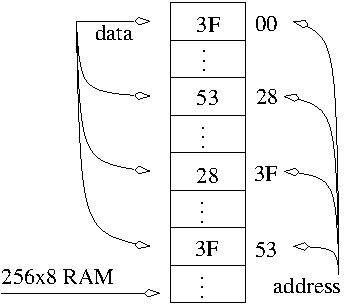
\includegraphics{Prob8-7}}
\caption{A 256x8 RAM loaded with some data.}
\label{fig:RAMhopper}
\end{figure}

\item \textbf{ (16 pts.)}
A 256x8 RAM is full of data.  Design a circuit that jumps 
around in memory.   The current address should be stored in a
register called PC.  If the MSB of the fetched word is 1, then the 
remaining seven bits represent a 7-bit 2's complement number;  add these 
seven bits to the PC.  If the MSB of the fetched word is 0 then just 
increment the PC.  Repeat this process forever.
Turn in; an algorithm the datapath and control unit, the control word 
table, the memory input equations, and output equations.  
The control unit is to be implemented using a ones hot encoding.

The desired behavior of the circuit is illustrated in 
Figure~\ref{fig:RAMhopper2}.  In this figure if PC=0 then the word at
that address (3F) has a MSB of 0 so the PC is incrementde to 1. The
word at address 1 is fetched (BC) and has an MSB of 1 so the least
significant seven bits of BC are added to the PC, making its new value
3D.  repeating this process sees the PC goto address 21, 22, 21, 22
into a never ending cycle.   Make sure the solution identifies how
to add the least significant seven bits to an 8-bit PC.

\begin{figure}[ht]
\center{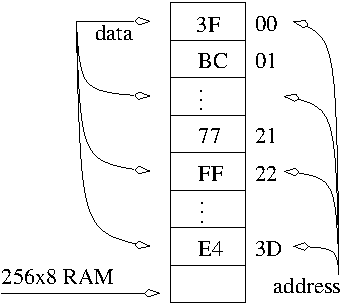
\includegraphics{Prob8-8}}
\caption{A 256x8 RAM loaded with some data.}
\label{fig:RAMhopper2}
\end{figure}

\begin{onlysolution}  \textbf{Solution} \itshape{

\begin{figure}[ht]
\center{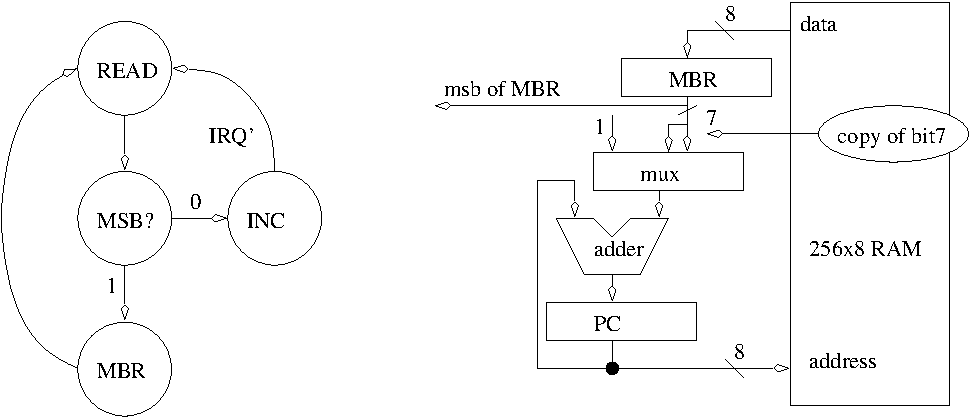
\includegraphics{Sol8-8}}
\caption{The datapath and control to conditionally hop around
in RAM.}
\end{figure}


\textbf{ Control Word}

\begin{tabular}{l|l|l|l|l|l|l}
STATE & RE     & CS     &MUX          &MBR    & PC	\\ \hline
      & 0 nada & 0 nada &0 pass 1     &0 hold &0 hold	\\ \hline
      & 1 read & 1 RAM  &1 pass MBR   &1 load &1 load	\\ \hline
      &        &        &             &       &       	\\ \hline
READ  & 1      & 1      & x           & 1     & 0	\\ \hline
MSB?  & 0      & 0      & x           & 0     & 0	\\ \hline
INC   & 0      & 0      & 0           & 0     & 1	\\ \hline
MBR   & 0      & 0      & 1           & 0     & 1	\\ \hline
\end{tabular}

\textbf{ MIEs and OEs}

\begin{tabular}{ll}
MIE					&	OE			\\
$D_{read}= Q_{mbr}+Q_{inc}$		&  $Z_{re} = Q_{read}$		\\
$D_{msb} = Q_{read}$			&  $Z_{cs} = Q_{read}$		\\
$D_{inc}= Q_{msb} m'$			&  $Z_{MUX} = Q_{mbr}$		\\
$D_{mbr}= Q_{msb} m$			&  $Z_{mbr} = Q_{read}$		\\
\end{tabular}

} \end{onlysolution} 


\item \textbf{ (16 pts.)}
Modify the circuit in the previous problem as follows.  Anytime
an external input, called IRQ, is asserted the circuit is to stop
jumping around and assert and ACK.  The outside world will then read
the PC (which must be routed outside the datapath) and then drop the 
IRQ.  The circuit should then drop the ACK and resume jumping.
Turn in; an algorithm the datapath and control unit, the control word 
table, the memory input equations, and output equations.  
The control unit is to be implemented using a ones hot encoding.


\item  \textbf{ (16 pts.)} Design a circuit that reads successive words from 
a 1kx12 RAM and
updates a 12-bit register called \textbf{ ACC} based on the upper two bits of the 
memory word.  The address of the current memory word should be contained
in a register called PC (Program Counter).  Since the words read from the
RAM will tell us what operation to perform on the ACC, the memory word will
be stored in a register called IR (Instruction Register).  If the upper
two bits of IR are:
\begin{enumerate}
\item  00 then add the lower 10 bits of the IR to ACC.  Pad the upper two
	bits of the IR with 0's before adding to the ACC.
\item  01 then store the ACC to the address specified by the 
	lower 10 bits of the IR.
\item  10 then load the ACC from from the address specified by the lower 
	10 bits of the IR.
\item  11 then clear the value of ACC to 0.
\end{enumerate}

The PC is to be initialized to 0.  After the each memory word is read
and the appropriate operation performed on ACC, the PC should be
incremented.
Turn in; an algorithm the datapath and control unit, the control word 
table, the memory input equations, and output equations.  
The control unit is to be implemented using a ones hot encoding.


\begin{onlysolution}  \textbf{Solution} \itshape{ 

\textbf{ Algorithm}
%% \begin{verbatim}
%% PC = 0;
%% while(1) {
    %% IR = RAM[PC];
    %% if (IR(11,10) == 00) 
	%% ACC += 00 & IR(9 downto 0);
    %% if (IR(11,10) == 01) 
	%% RAM[IR(9 downto 0) = ACC;
    %% if (IR(11,10) == 10) 
	%% ACC = RAM[IR(9 downto 0)];
    %% if (IR(11,10) == 11) 
	%% ACC = 0;
    %% PC += 1;
%% }
%% \end{verbatim}

\textbf{ Datapath and Control}

\begin{figure}[ht]
\center{\scalebox{0.7}{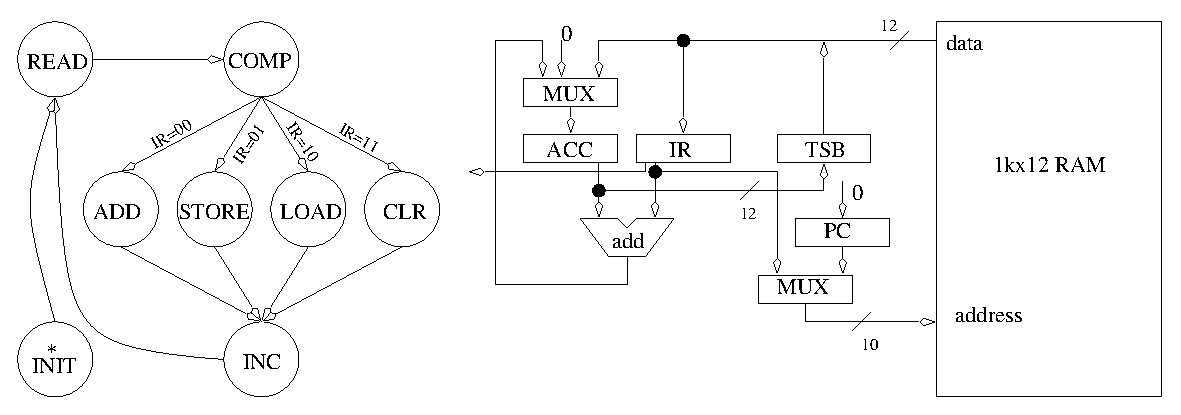
\includegraphics{Sol8-10}}}
\end{figure}

\textbf{ Control Word}

\tiny{
\begin{tabular}{l|l|l|l|l|l|l|l|l}
State & ACC mux	& Acc   & IR    & TSB   & PC	    & Addr Mux & CS	& R/W'	\\ \hline
      & 00 add & 0 hold & 0 hold & 0 Z    & 00 hold & 0 PC	& 0 no & 0 write \\ \hline
      & 01 0   & 0 load & 0 load & 1 pass & 01 load & 1 IR	& 0 on & 1 read \\ \hline
      & 10 RAM & 	& 	& 	& 10 up	&	 	& 	 & 	\\ \hline
      & 	& 	& 	& 	& 	& 	 	& 	 & 	\\ \hline
Init  &	01	& 1	& 0	& 0	& 01	&	x	& 0	& x	\\ \hline
Read  & xx	& 0	& 1	& 0	& 00	&	0	& 1	& 1	\\ \hline
Comp  & xx	& 0	& 0	& 0	& 00	&	x	& 0	& x	\\ \hline
Add   & 00	& 1	& 0	& 0	& 00	&	x	& 0	& x	\\ \hline
Stor  & xx	& 0	& 0	& 1	& 00	&	1	& 1	& 0	\\ \hline
Load  & 10	& 0	& 0	& 0	& 00	&	1	& 1	& 1	\\ \hline
Clr   & 01	& 1	& 0	& 0	& 00	&	x	& 0	& x	\\ \hline
Inc   & xx	& 0	& 0	& 0	& 10	&	x	& 0	& x	\\ 
\end{tabular}
}


\textbf{ MIEs and OEs}

\begin{tabular}{ll}
MIE                                     &       OE                      \\
$D_{Init}= Q_{wait1a}req'$            &  $Z_{m1} = Q_{load}$           \\
$D_{Read } = Q_{wait1a}req$             &  $Z_{Init} = Q_{Clr}$           \\
$D_{Comp}= Q_{getA} + Q_{wait2A}req$  &  $Z_{Acc} = Q_{Init} + Q_{Add} + Q_{Clr}$               \\
$D_{Add}= Q_{wait2a}req' + Q_{wait1B}req'$   &  $Z_{IR} = Q_{Read}$     \\
$D_{Stor} = Q_{wait1b}req$             &  $Z_{TSB} = Q_{Stor}$         \\
$D_{Load}= Q_{GetB} + Q_{wait2b}req$  &  $Z_{PC1} = Q_{Inc}$          \\
$D_{Clr  } = Q_{wait2B}req'$            &  $Z_{PC0} = Q_{Init}$          \\
$D_{Inc } = Q_{For}LB$                 &   $Z_{CS} = Q_{Read}+Q_{Stor}+Q_{Load}$     \\
					&   $Z_{Amux} = Q_{Read}+Q_{Stor}+Q_{Load}$   \\
					&   $Z_{RW} = Q_{Read}+Q_{Load}$            \\
\end{tabular}

}\end{onlysolution} 

\item \textbf{ (16 pts.)}
Design a circuit that moves $M$ consecutive words from address $S$ (source) to
address $D$ (destination).  For example, if $M=4$, $S=3EA$ and $D=1FE$ then the 
circuit would move words 3EA, 3EB, 3EC and 3ED to address 1FE, 1FF, 200 and 201.
Each of $M,S,D$ is preloaded into a register.  While this problem appears simple,
its really rather treacherous.  The circuit will have to handle cases where 
$S+M > D$.  In such a case the order of the data movement must be carefully planned.
In order to simplify the design, assume that $S<D$.  
Turn in; an algorithm the datapath and control unit, the control word 
table, the memory input equations, and output equations.  
The control unit is to be implemented using a ones hot encoding.
Do not worry about the sizes of the
registers or RAM.

\item \textbf{ (16 pts.)}
Design a circuit that determines how many times a user
specified 8-bit value, called \textbf{ key}, occurs in an 1kx8 RAM.  
\textbf{ key} is to be read using a two-line handshake; the circuit 
is the passive consumer.
Turn in; an algorithm the datapath and control unit, the control word 
table, the memory input equations, and output equations.  
The control unit is to be implemented using a ones hot encoding.


\item \textbf{ (16 pts.)} Design a circuit that records the number of times that it
has seen an 8-bit, user specified value, \textbf{ key}.  The key will
is shown to the circuit, at most, 16 times.  The collection of 
keys is stored in a 1kx12 RAM.  The RAM is larger
than it needs to be because it is thought that in the future
the number of keys will be increased.  Each word of the RAM is 
organized as follows; The upper eight bits hold the key and the lower
four bits hold the ``hit count", the number of times that this key has
been seen.  The circuit should read in the key using a two-line
handshake; the circuit is the passive consumer.  The circuit
should then scan the RAM looking for a matching key; a match, if
it exists, will only occur once in the RAM.  If a match is 
found then increment the lower four bit and store the key and the
incremented hit count back to RAM.  
Turn in; an algorithm the datapath and control unit, the control word 
table, the memory input equations, and output equations.  
The control unit is to be implemented using a ones hot encoding.


\item \textbf{ (36 pts.)}
Design a digital circuit to control access to an
automated parking garage containing 828 parking spaces.  
Drivers pull up to the garages gate and insert 
their pass card into a card reader.  The card reader sends the pass card
ID number to the digital circuit.  If their pass card has a valid
code then the gate opens.  There is a pressure sensor just inside the
entry way which sends a signal to the circuit whenever a significant
load is present (over 150 lbs).
The exit procedure is similar, the users have to insert their pass card
into a card reader.  The digital circuit then raises the exit gate bar,
a pressure sensor at the exit tells the circuit when it is OK to close
the exit gate.  See Figure~\ref{fig:Garage}.
\begin{figure}[ht]
\center{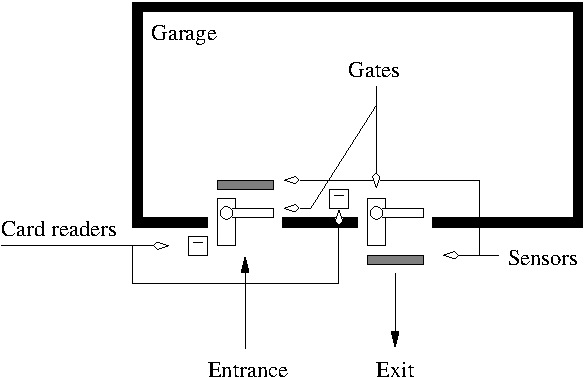
\includegraphics{Prob8-14}}
\caption{The layout of an automated garage.}
\label{fig:Garage}
\end{figure}

The signal names are defined in the following table:

\begin{tabular}{|l|l||l|l|} \hline
Entrance gate	& InGate	& 0 Close gate & 1 Open gate \\ \hline
Entrance sensor	& InSen		& 0 No weight &  1 Weight present \\ \hline
Entrance REQ	& InREQ		& 0 No card read data & 1 Card reader has data  \\ \hline
Entrance ACK	& InACK		& \multicolumn{2}{c|}{Circuit control}   \\ \hline
Entrance ID	& InID		& \multicolumn{2}{c|}{Card ID} \\ \hline
Exit gate	& OutGate	& 0 Close gate &  1 Open gate \\ \hline
Exit sensor	& OutSen	& 0 No weight & 1 Weight present\\ \hline
Exit REQ	& OutREQ	& 0 No card read data & 1 Card reader has data  \\ \hline
Exit ACK	& OutACK	& \multicolumn{2}{c|}{Circuit control}   \\ \hline
Exit ID		& OutID		& \multicolumn{2}{c|}{Card ID} \\ \hline
\end{tabular}

The gate requires a logic 1 to start and to stay open. The sensor will 
generate a logic 1 while there is more than 150 lbs. on the sensor.  Only
close the gate when the rear wheels of the car activate the
sensor (hope no unicycle use the garage).  The entrance card reader 
will provide InID or OutID using a 
two-line handshake, where the circuit is the passive consumer.
Assume that at any point in time only one car is
entering or leaving the garage.  That is, deal with only
one direction at a time.

In addition to controlling access to the garage, the clients would also
like to keep track track of how many times a pass ID has been used to
gain access in-to and out-of the garage.  The count will be checked and
reset once a month.  Cars pass into and out of the garage at most 4
times a day.

To implement this circuit use a \textit{ single} RAM.  Each word of the
RAM must be divided into three fields; ID, Ins and Outs corresponding to
the pass ID number, number of times into the garage and number of times
out of the garage respectively.   The digital circuit will scan successive
IDs in the RAM looking for a match.  If a match 
is found then either increment the Ins or Outs field then store this 
item back into the RAM.  A major issue in this design is determining
the sizes of the data items.  Use the information in the word statement
to make the design as space efficient as possible.
\begin{figure}[ht]
\center{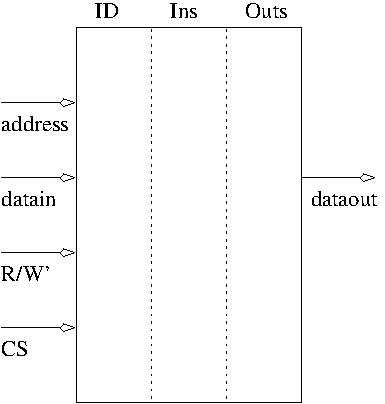
\includegraphics{Prob8-14b}}
\caption{The format of the RAM in the garage circuit problem.}
\label{fig:GarRAM}
\end{figure}
Turn in; an algorithm the datapath and control unit, the control word 
table, the memory input equations, and output equations.  
The control unit is to be implemented using a ones hot encoding.


\item \textbf{ (16 pts.)} Design a circuit that converts a 6-bit binary number into a 2 
digit BCD representation.  The circuit acquires a 6-bit number through
a two-line handshake where the circuit is a passive consumer.  The 
circuit is then to convert this 6-bit number into two BCD digits and
signals it completion via a DONE signal.

A number X can be converted from binary into BCD digits by iteratively
checking that X is greater than 10, then subtracting 10 from X.  Each
subtraction should increment a tens digit counter.

Make sure to identify the size of all the signals in the datapath
and the size of any register, counters, etc...
Turn in; an algorithm the datapath and control unit, the control word 
table, the memory input equations, and output equations.  
The control unit is to be implemented using a ones hot encoding.

 
\item \textbf{ (8 pts.)}
Design a circuit that converts a 2 digit BCD number into a
binary number.  The circuit acquires the BCD digits through 2 read
operations most significant digit first.  Each read operation takes 
the form of a two-line handshake where the circuit is a passive 
consumer.

A 2 digit BCD number can be converted into binary by multiplying the
most significant digit by 10 then adding it to the least significant
BCD digit.  A number can be multiplied by 10 using the shift-and-add
technique presented on page~\pageref{page:MulyBy10}.  Note, this
task can be accomplished without using a single shift register.
For example, the adder in Figure~\ref{fig:NineTimes} generates the value
of 9*X from a 4-bit register by adding X, shifted left by three bits, to X.

\begin{figure}[ht]
\center{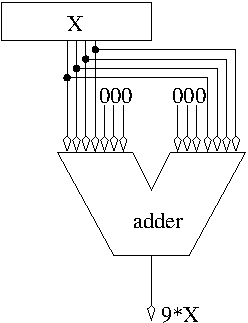
\includegraphics{Prob8-16}}
\caption{A simple circuit to compute 9*X.}
\label{fig:NineTimes}
\end{figure}

Make sure to identify the size of all the signals in the datapath
and the size of any register, counters, etc...
Turn in; an algorithm the datapath and control unit, the control word 
table, the memory input equations, and output equations.  
The control unit is to be implemented using a ones hot encoding.

 
\item \textbf{ (36 pts.)}
Design a digital circuit that plays a game of
roulette, allows betting and keeps track of total earnings.
The roulette wheel has 8 slots, labeled $1 \ldots 8$.  The player
can play one of the numbers straight or play even or odd.
The player starts with \$10. 
The layout of the machine is shown in Figure~\ref{fig:Roulette}.
\begin{figure}[ht]
\center{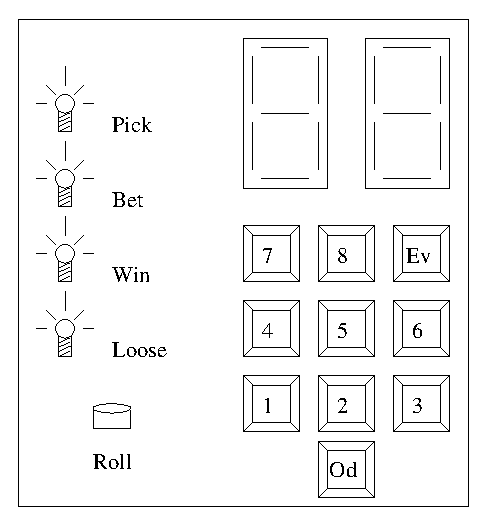
\includegraphics{Prob8-17}}
\caption{The layout of the roulette playing machine.  
The two 7-segment displays at the top are used for a variety
of purposes.}
\label{fig:Roulette}
\end{figure}

The sequence of events is as follows:
\begin{enumerate}
\item	The circuit lights up the PICK LED.
	The player enters their guess; a number between 1-8, even or odd.
	While holding down their guess they press the roll button.
\item	The circuit displays the picked number in the left most
	7-segment display.  The circuit lights up the BET LED.
	The player enters a one digit bet between 1 to 8.  While holding
	down their bet they press the roll button.
\item 	The circuit displays the bet on the rightmost 7-segment
	display.
	The player pushes and holds down the roll button.
	The circuit increments a mod 8 counter while the roll 
	button is depressed. It would be nice to display the
	current count value on right 7-seven segment display.
	Since the clock cycle is on the order of milliseconds,
	then the user would not be able to anticipate the roll.
\item	The player releases the roll button.  The final roll
	is displayed on the rightmost 7-segment display.
	The circuit stops incrementing the counter and checks
	to see if the final value matches the players guess.
	If the match is correct then light the WIN LED and
	increment the players earnings.  If the match is incorrect
	then light the LOOSE LED and decrement the players
	earnings.
\item	The play hits the roll button to clear the roll information
	from the 7-segment displays.
\item	The circuit displays the players earnings on the 7-segment
	display.
\item	When the user pushes the roll button then go to step 1.
\end{enumerate}

Set reasonable bounds on the maximum winnings.  Values may be displayed
in hexadecimal (assume there is a hex to 7-segment display converter
available).  See page~\pageref{page:7seg} for more
information.
Turn in; an algorithm the datapath and control unit, the control word 
table, the memory input equations, and output equations.  
The control unit is to be implemented using a ones hot encoding.


\begin{onlysolution}  \textbf{Solution} \itshape{

\textbf{ Algorithm}

%% cash = 10; 
%% left_seven = blank; 
%% right_seven = cash; 
%% while(cash > 0) { 
%%     led_array = 1 0 0 0;    // Pick Bet Win Loose 
%%     while(ROLL == 0); 
%%     guess = Datain; 
%%     while(ROLL == 1); 
%%      
%%     led_array = 0 1 0 0;    // Pick Bet Win Loose 
%%     left_seven = guess; 
%%     right_seven = blank; 
%%     while(ROLL == 0); 
%%     bet = Datain; 
%%     while(ROLL == 1); 
%%      
%%     led_array = 0 0 0 0;    // Pick Bet Win Loose 
%%     right_seven = bet; 
%%     while(ROLL == 0); 
%%     while(ROLL == 1) count = count + 1; 
%%  
%%     right_seven = count; 
%%     if (count == guess) { 
%%         cash = cash + (bet << 2); 
%%         led_array = 0 0 1 0;    // Pick Bet Win Loose 
%%     } else { 
%%         cash = cash - bet; 
%%         led_array = 0 0 0 1;    // Pick Bet Win Loose 
%%     } 
%%     while(ROLL == 0); 
%%     while(ROLL == 1); 
%%     right_seven = cash; 
%%  
%% }	 
%% led_array = 0 0 0 1;    // The user is out of money 
%% while(1);		// Halt the machine 
 
\textbf{ Datapath and Control}

\begin{figure}[ht]
\center{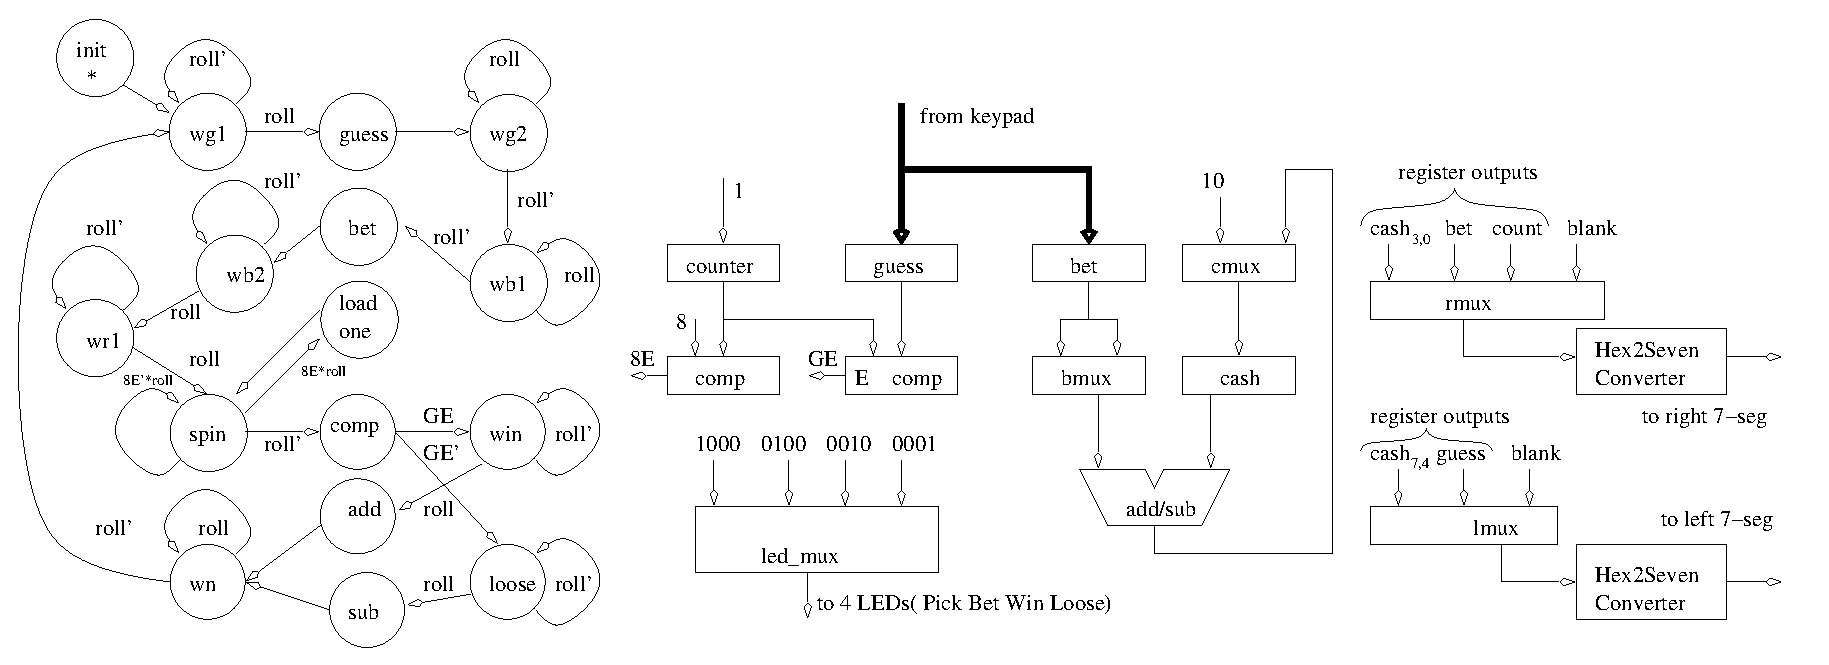
\includegraphics{Sol8-16}}
\end{figure}

Note from the figure that, the user may acquire
up to 0xFF cash.  Each hex digit of the users total cash will 
be displayed on its own 7-segment display.

\textbf{ Control Word}

{\tiny
\begin{tabular}{l|l|l|l|l|l|l|l|l|l|l}
State &  counter& guess  & bet    & cmux      & bmux     & cash   & add/sub & ledmux    & rmux   & lmux \\ \hline
      & 00 hold & 0 hold & 0 hold & 0 \$10    & 0 bet    & 0 hold & 0 add  & 00 (pick) &00 cash &00 cash  \\ \hline
      & 01 load & 0 load & 1 load & 1 add/sub & 1 bet<<2 & 1 load & 1 sub  & 01 (bet ) &01 bet  &01 guess \\ \hline
      & 10 up   &        &        &  	      &          &        &        & 10 (win ) &10 count&10 blank \\ \hline
      &         &        &        &  	      &          &        &        & 11 (loose)&11 blank&         \\ \hline
      &         &        &        &  	      &          &        &        &          &         &   \\ \hline
init  & 00      & 0      &  1     & 0	      & x        &  1     &  x     & 00       &  11     & 11\\ \hline
wg1   & 00      & 0      &  0     & x	      & x        &  0     &  x     & 00       &  00     & 00\\ \hline
guess & 00      & 1      &  0     & x	      & x        &  0     &  x     & 00       &  11     & 01\\ \hline
wg2   & 00      & 0      &  0     & x	      & x        &  0     &  x     & 00       &  11     & 01\\ \hline
wb1   & 00      & 0      &  0     & x	      & x        &  0     &  x     & 01       &  11     & 01\\ \hline
bet   & 01      & 0      &  1     & x	      & x        &  0     &  x     & 01       &  11     & 01\\ \hline
wb2   & 00      & 0      &  0     & x	      & x        &  0     &  x     & 00       &  01     & 01\\ \hline
wr1   &         &        &        & x	      & x        &        &  x     &          &         &   \\ \hline
spin  & 10      & 0      &  0     & x	      & x        &  0     &  x     & 00       &  10     & 01\\ \hline
load 1& 01      & 0      &  0     & x	      & x        &  0     &  x     & 00       &  10     & 01\\ \hline
comp  & 00      & 0      &  0     & x	      & x        &  0     &  x     & 00       &  10     & 01\\ \hline
win   & 00      & 0      &  0     & 1	      & 1        &  1     &  0     & 10       &  10     & 01\\ \hline
add    &         &        &        &  	      &          &        &        &          &         &   \\ \hline
loose & 00      & 0      &  0     & 1	      & 0        &  1     &  1     & 11       &  10     & 01\\ \hline
sub   &         &        &        &  	      &          &        &        &          &         &   \\ \hline
wn    & 00      & 0      &  0     & x	      & x        &  0     &  x     & 00       &  00     & 00\\ 
\end{tabular}
}

\textbf{ MIEs and OEs}

$$
\begin{array}{ll}
MIE						&       OE                      \\
D_{init}= 0					&  Q_{c1} = Q_{spin}          \\
D_{wg1}= Q_{wg1}*roll'+Q_{wn}*roll'		&  Z_{c0} = Q_{bet} + Q_{load1}           \\
D_{guess} = Q_{wg1}*roll           		&  Z_{guess} = Q_{guess}           \\
D_{wg2}= Q_{guess} + Q_{wg2}*roll		&  Z_{bet}= Q_{init} + Q_{bet} \\
D_{wb1}= Q_{wg2}*roll'+Q_{wb1}*roll		&  Z_{cmux} = Q_{win}+Q_{loose}           \\
D_{bet } = Q_{wb1}*roll'			&  Z_{bmux} = Q_{win}           \\
D_{wb2}= Q_{bet} + Q_{wb2}*roll'		&  Z_{cash} = Q_{init} + Q_{win} + Q_{loose}    \\
D_{spin}= Q_{wb2}roll + Q_{spin}*8E'roll + Q_{load1}  &  Z_{addsub} = Q_{loose}     \\
D_{load1}= Q_{spin}*8E*roll    		& Z_{led1} = Q_{win} + Q_{loose} \\
D_{comp} = Q_{spin}roll'			& Z_{led0} = Q_{wb1}+Q_{bet}+Q{loose}         \\
D_{win}= Q_{comp}*GE				& Z_{rseg1} = not (Q_{wg1}+Q_{wb2}+Q_{wn})      \\
D_{loose} = Q_{comp}*GE'			& Z_{rseg0} = Q_{init,guess,wg2,wb1,bet,wb2}\\
D_{wn2} = Q_{wn}*roll + Q_{win}*roll + Q_{loose}*roll & Z_{lseg1} = Q_{init}  \\
\end{array} $$

} \end{onlysolution} 

\item \textbf{ (20 pts.)}
Design a tone generator.  The tone generator is a box with two buttons
on it labeled ``Up" and ``Down" and a 1-bit output.  At start-up the tone 
generator outputs
a 440Hz square wave (clock-like signal).  Every time that the Up button
is pressed the tone generator should increase the frequency of the square
wave by $\sqrt[12]{2}-1.0 = 0.059463094 \approx 7/128$ of its current frequency.  
To determine the fraction $7/128$ of $X$, shift $X$ left by 7-bits (dividing by
128) then multiplying it by 4+2+1.  Every time that the down button is pressed
the circuit should decrease the frequency by 7/128 of its current value.  Assume
that the master clock frequency of the circuit is 4Mhz.  Turn in 
any relevant calculations, algorithm, datapath and control, control word,
MIEs, OEs and the maximum tone frequency of the circuit.
Turn in; an algorithm the datapath and control unit, the control word 
table, the memory input equations, and output equations.  
The control unit is to be implemented using a ones hot encoding.


\end{enumerate}
